%!TEX root = ../main.tex


\section{Approach Description} 
\label{sec:sys}
%-------------------------------------------%

In this section, we describe our rule learning system with embedding support. 
Conceptually, 
it extends the standard relational association rule learners \cite{amie,DBLP:conf/esf/GoethalsB02} to also take into account the feedback from embedding models through the probabilistic function $f$. 

Following common practice~\cite{amie} we restrict ourselves to rules that are \emph{closed}, where every variable appears at least twice (moreover, we extract only rules whose Horn part is \emph{closed}), and \emph{safe}, where variables appearing in the negated part also appear in the positive part of the rule.

\begin{figure}[t]
\centering
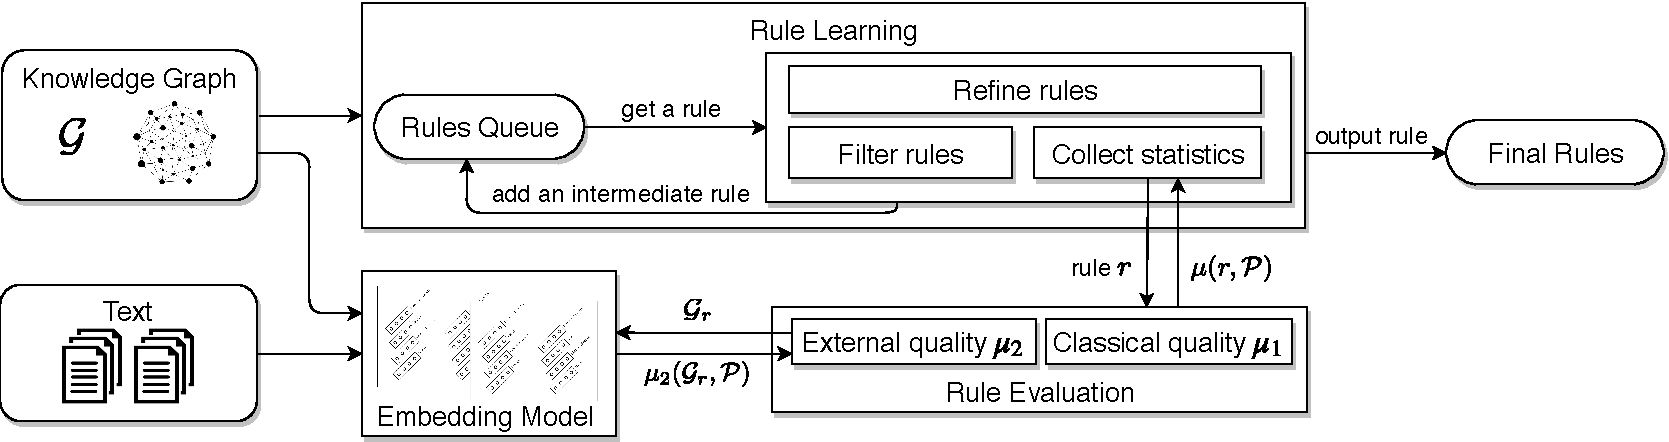
\includegraphics[width=1\textwidth]{figures/system_overview_H.pdf}
\caption{Overview of our system.}
\label{fig:system}
\end{figure}


\subsubsection{Overview.}
%------------------------------------------%
The input of the system are a KG, possibly a text corpus, and a set of user specified parameters that are used to terminate rule construction.
These parameters include an embedding weight $\lambda$, 
a minimum threshold 
for $\mu_1$,  
a minimum rule support $\textit{r-supp}$ 
and other \emph{rule-related} parameters such as a maximum number of positive 
and negative 
atoms allowed in $r$.
The KG and text corpus are used to train the embedding model that in turn is used to construct the probabilistic function $f$.
The rules $r$ are constructed in the iterative fashion, starting from the head, by adding atoms to its body one after another until at least one of the termination criteria (that depend on $f$) is met.
In parallel with the construction of the rule $r$, the quality $\mu(r)$ is computed.
\thi{question from reviewer: how are atoms selected, exactly?}

In Figure~\ref{fig:system} we present a high level architecture of our system, where arrows depict information flow between blocks.
The \emph{Rule Learning} block constructs rules over the input KG, \emph{Rule Evaluation} supplies it with quality scores $\mu$ for rules $r$, using $\cG$ and $f$, where $f$ is computed by the \emph{Embedding Model} block 
from $\cG$ and text.




We now discuss the algorithm behind the \emph{Rule Learning} block
in Figure~\ref{fig:system}. 
Following \cite{amie} we model rules as sequences of atoms, where the first atom is the head of the rule and other atoms are its body. 
The algorithm maintains a priority queue of intermediate rules
(see the \emph{Rules Queue} block in Figure~\ref{fig:system}). 
Initially all possible binary atoms appearing in $\cG$ are added to the queue with empty bodies. 
At each iteration, a single rule is selected from the queue. 
If the rule satisfies the \emph{filtering criteria} 
(see the \emph{Filer rules} block) 
which we define below,
then the system returns it as an output. 
If the rule is not filtered, then it is processed with one of the \emph{refinement operators} 
(see the \emph{Refine rules} block) 
that we define below that expand the rule with one more atom 
and produce new rule candidates, 
which are then pushed into the queue 
(if not being pushed before). 
The iterative process is repeated until the queue is empty. 
All the reported rules will be finally ranked by the decreasing order of the hybrid measure $\mu$, computed in \emph{Collect statistics} block.

In the remainder of the section we discuss refinement operators and filtering criteria.
 


\subsubsection{Refinement operators.}
%------------------------------------------%
We rely on the following three standard refinement operators \cite{amie}
that extend rules:
\begin{enumerate}[label=(\it\roman*)]
\item \textit{add a positive dangling atom}: add a binary positive atom with one fresh variable and another one appearing in the rule, i.e., \emph{shared}.
\item \textit{add a positive instantiated atom}: add a binary positive atom with one argument being a constant and the other one being a shared variable.
\item \textit{add a positive closing atom}: add a binary positive atom with both of its arguments being shared variables.
\end{enumerate}

Additionally, we introduce two more operators to allow negated atoms in rule bodies: 

\begin{enumerate}
\item[\it (iv)] \textit{add an exception instantiated atom}: add a binary negated atom with one of its arguments being a constant, and the other one being a shared variable. 
\item[\it (v)] \textit{add an exception closing atom}: add a binary negated atom to the rule with both of its arguments being shared variables.% 
\end{enumerate}
%
These two operators are only applied to closed rules. 
Moreover, we ensure that the addition of exception atoms to the rule $r:\mi{head(r)\leftarrow body^+(r)}$, 
should result in $r': \mi{head(r)\leftarrow body^+(r), \naf body^-(r)}$, such that 
\[\textit{r-supp}(\mi{head(r)\leftarrow body^+(r), body^-(r)},\cG)=0.\]
Intuitively, we aim at adding exceptions  
that explain the absence of predictions expected to be in the graph rather then their presence. Thus, the introduced exceptions should not affect the rule support, i.e., $\textit{r-supp}(r,\cG) = \textit{r-supp}(r',\cG)$. 

\subsubsection{Filtering criteria.}
%------------------------------------------%
After applying one of the refinement operators to a rule, 
a set of candidate rules is obtained. 
For each candidate rule we first verify that the hybrid measure $\mu$ has increased and discard the rule if it has not. 
Then, we compute its \emph{h-cover}~\cite{amie} and our novel exception confidence measure \emph{e-conf} that are defined as follows:
\begin{align*}
	\textit{h-cover}(r,\cG) & =
		\textit{r-supp}(r,\cG)/
		|\set{h \mid 
				h(head(r,\cG)) \in \G}|,\\
	\textit{e-conf}(r,\cG) & =
		\textit{conf}(r'',\cG),
\end{align*}
where $r'':body^-(r)\leftarrow body^+(r), not\;head(r)$.
If the \emph{h-cover} and \emph{e-conf} are below the user specified threshold, then the rule is discarded.
Intuitively, \emph{h-cover} quantifies the ratio of the known true facts that are implied by the rule.
In contrast, \emph{e-conf} is the conditional probability of the exception given predictions produced by the Horn part of $r$, which helps to disregard insignificant exceptions, i.e., those that explain the absence in $\cG$ of only a small fraction of predictions made by $\mi{head(r)}\leftarrow \mi{body^+(r)}$, as such exceptions likely correspond to noise. 
%
Observe that not all of the filtering criteria are relevant for all rule types. For example, exception confidence is relevant only for non-monotonic rules to ensure the quality of the added exceptions.

Finally, note that by exploiting the embedding feedback, we can now distinguish exceptions from noise. 
Consider the rule stating that married people live together.  This rule can have several possible exceptions, e.g., either one of the spouses is a researcher or he/she works at a company, which has headquarter in the US. Whenever the rule is enriched with an exception, naturally, the support of its body decreases, i.e., the size of $\cG_r$ goes down. 
Relying on our filtering criteria, we aim at 
adding such negated atoms, that the average quality of $\cG_r$ increases, meaning that the introduced negated atoms prevent unlikely predictions.



